\chapter{AWS Deployment \\
\small{\textit{-- Justin Baumann, Gianna Cerbone, Thomas Ung, Spurthi Setty}} 
\index{Chapter!AWSDeployment}
\index{AWSDeployment}
\label{Chapter::AWS Development}}

\section{Overview}
These instructions are for a Windows machine, assuming Docker and AWS CLI are already installed and an AWS account has been created. These are step-by-step instructions to:
\begin{enumerate}
  \item Configure AWS CLI with IAM Identity Center (SSO).
  \item Push a Docker container image to Amazon Elastic Container Registry (ECR).
  \item Deploy the container image to AWS App Runner.
\end{enumerate}

\section{Set up Environment}
\begin{enumerate}
    \item Ensure that Docker Desktop is installed and open the application 
    \item Open command prompt and navigate to the directory which contains the Dockerfile for the color button app. 
    \item Verify installation of AWS CLI by running the following in your command prompt 
    \begin{minted}
        [fontsize=\small,breaklines]{bash}
        aws --version
    \end{minted}
    You should get an output something like 
    \begin{minted}
        [fontsize=\small,breaklines]{bash}
        aws-cli/2.15.54 Python/3.11.8 Windows/10 exe/AMD64
    \end{minted}
    
\end{enumerate}

\section{Set up IAM Identity Center}
\begin{enumerate}
    \item Login into you AWS Console 
    \item Navigate to IAM Identity Center, and click enable 
    \item On the left hand menu, click on Users and then the Add User button on the top right
    \item Enter the specified username, email and Name. I created a user with the following information 
    \begin{itemize}
        \item username: spurthi
        \item email: spurthi.setty@gmail.com
        \item Display name: Spurthi Setty 
    \end{itemize}
    \item Click on next - no need to fill out additional information or add the user to a group
    \item Select your preferred method of creating a password, I used a one time code, and set up 2FA with my Microsoft authenticator app. 
    \item Follow instructions to verify your email for your user
    \item In your user, click on the tab for AWS Accounts, and then the button called Assign Accounts
    \item Click on Create permissions set $\rightarrow$  predefined $\rightarrow$ Administrator Access 
    \item Assign the access for your user and wait for the confirmation message
    \item Go back to AWS $\rightarrow$ IAM Identity Center $\rightarrow$ Settings. Here you should see a AWS access portal URL. This is your SSO Start URL for the next section. For me it was 
\begin{minted}[fontsize=\small,breaklines]{bash}
https://d-906629391d.awsapps.com/start
\end{minted}
\end{enumerate}



\section{Configure AWS CLI with SSO}
\begin{enumerate}
    \item Run the following command 
\begin{minted}[fontsize=\small,breaklines]{bash}
aws sso login
\end{minted}
    \item You will be prompted to enter a series of inputs, here are the values to provide
    \begin{itemize}
      \item SSO session name: my-sso (or any name)
      \item SSO start URL: https://d-906629391d.awsapps.com/start (or whatever you AWS Access portal URL is)
      \item SSO region: us-east-1
      \item SSO registration scopes: (blank)
    \end{itemize}
    \item The browser will open the url, and the command prompt will aslo provide the URL to an SSO authorization page. 
    \item Enter the username and password on the page for the user you created in the previous section. 
    \item You will then be asked to input a 6 digit code on your browser from you command prompt, or asked to confirm the code.
    \item Approve any permissions and you should get a confirmation message that your request has been approved. 
    \item  You can now close this tab from your browser 
    \item Confirm you have sucessfull logged in by running the following command 
    \begin{minted}[fontsize=\small,breaklines]{base}
        aws sts get-caller-identity
    \end{minted}
    \item Ensure that you are logged in as the user you created with admistrator access. If you are not, then try the sso command again. An example of the expected output for the previous step is
    \begin{minted}[fontsize=\small,breaklines]{json}
    {
    "UserId": "AROAW4ZMTTNJFUQ2BGYAX:spurthi",
    "Account": "474150574930",
    "Arn": "arn:aws:sts::474150574930:assumed-role/AWSReservedSSO_AdministratorAccess_67ee4a10fe53d47e/spurthi"
    }
    \end{minted}
\end{enumerate}


\section{Set Environment Variables (Windows CMD)}

Run the following commands, adjusting names and values are needed. the AWS\_ACCOUNT\_ID should correspond to the value for account in the previous step. The CONTAINER\_PORT should correspond to whatever port is specified in you Dockerfile.
\begin{minted}[fontsize=\small,breaklines]{bat}
set AWS_REGION=us-east-1
set AWS_ACCOUNT_ID=474150574930
set ECR_REPO=color-buttons-app
set IMAGE_TAG=v1
set CONTAINER_PORT=3000
set APP_NAME=my-apprunner-app
\end{minted}

\section{Create an ECR repository}
\begin{enumerate}
    \item Run the following command to describe and create an ECR repository 
    \begin{minted}[fontsize=\small,breaklines]{bat}
    aws ecr describe-repositories --repository-names %ECR_REPO% --region %AWS_REGION% >NUL 2>&1 || ^
    aws ecr create-repository --repository-name %ECR_REPO% --image-scanning-configuration scanOnPush=true --region %AWS_REGION%
    \end{minted}
    \item The output should look something like this\begin{minted}[fontsize=\small,breaklines]{json}
    {
        "repository": {
            "repositoryArn": "arn:aws:ecr:us-east-1:474150574930:repository/color-buttons-app",
            "registryId": "474150574930",
            "repositoryName": "color-buttons-app",
            "repositoryUri": "474150574930.dkr.ecr.us-east-1.amazonaws.com/color-buttons-app",
            "createdAt": "2025-09-29T21:43:04.517000-04:00",
            "imageTagMutability": "MUTABLE",
            "imageScanningConfiguration": {
                "scanOnPush": true
            },
            "encryptionConfiguration": {
                "encryptionType": "AES256"
            }
        }
    }
    \end{minted}
    \item Confirm that the ECR was created by checking it on your AWS console under Elastic Container Registry

\end{enumerate}



\section{Build, Tag, and Push Docker Image}
\begin{enumerate}
    \item Login to docker by running the following command
    \begin{minted}[fontsize=\small,breaklines]{bat}
    aws ecr get-login-password --region %AWS_REGION% | docker login --username AWS --password-stdin %AWS_ACCOUNT_ID%.dkr.ecr.%AWS_REGION%.amazonaws.com
    \end{minted}
    You should get a message that Login succeeded

    \item Build you Docker container by running the following command
    \begin{minted}[fontsize=\small,breaklines]{bat}
    docker build --platform linux/amd64 -t %ECR_REPO%:%IMAGE_TAG% .
    \end{minted}
    If successfull, you terminal should look something like 
    \begin{minted}[fontsize=\small,breaklines]{text}
[+] Building 1.3s (10/10) FINISHED            docker:desktop-linux
\end{minted}

    \item Tag it to your ECR by running the following command
    \begin{minted}[fontsize=\small,breaklines]{bat}
    docker tag %ECR_REPO%:%IMAGE_TAG% %AWS_ACCOUNT_ID%.dkr.ecr.%AWS_REGION%.amazonaws.com/%ECR_REPO%:%IMAGE_TAG%
    \end{minted}

    \item Push your docker container by running the following command 
    \begin{minted}[fontsize=\small,breaklines]{bat}
    docker push %AWS_ACCOUNT_ID%.dkr.ecr.%AWS_REGION%.amazonaws.com/%ECR_REPO%:%IMAGE_TAG%%
    \end{minted}
    If sucessfull, you should see these Images populate in your AWS console within this ECR

    \item Very that the image is pushed by running the following command 
    \begin{minted}[fontsize=\small,breaklines]{bat}
    aws ecr describe-images --repository-name %ECR_REPO% --region %AWS_REGION% --query "imageDetails[].imageTags"
    \end{minted}

    The output should look like this, with whatever you specified the image tag as: 
    \begin{minted}[fontsize=\small,breaklines]{json}
        [
            [
                "v1"
            ]
        ]
        \end{minted}

    
    
    
\end{enumerate}
\section{Create App Runner ECR Access Role}
\begin{enumerate}
  \item Create the role:
\begin{minted}[fontsize=\small,breaklines]{bat}
aws iam create-role --role-name AppRunnerECRAccessRole --assume-role-policy-document "{\"Version\":\"2012-10-17\",\"Statement\":[{\"Effect\":\"Allow\",\"Principal\":{\"Service\":\"build.apprunner.amazonaws.com\"},\"Action\":\"sts:AssumeRole\"}]}"
\end{minted}

  \item Attach the policy:
\begin{minted}[fontsize=\small,breaklines]{bat}
aws iam attach-role-policy --role-name AppRunnerECRAccessRole --policy-arn arn:aws:iam::aws:policy/service-role/AWSAppRunnerServicePolicyForECRAccess
\end{minted}

  \item Save the role ARN in an environment variable:
\begin{minted}[fontsize=\small,breaklines]{bat}
set ACCESS_ROLE_ARN=arn:aws:iam::%AWS_ACCOUNT_ID%:role/AppRunnerECRAccessRole
\end{minted}
\end{enumerate}

\section{Deploy with App Runner}
\begin{enumerate}
  \item Create the App Runner service:
\begin{minted}[fontsize=\small,breaklines]{bat}
aws apprunner create-service ^
--service-name %APP_NAME% ^
--region %AWS_REGION% --profile default ^
--source-configuration "{\"AuthenticationConfiguration\":{\"AccessRoleArn\":\"%ACCESS_ROLE_ARN%\"},\"ImageRepository\":{\"ImageIdentifier\":\"%AWS_ACCOUNT_ID%.dkr.ecr.%AWS_REGION%.amazonaws.com/%ECR_REPO%:%IMAGE_TAG%\",\"ImageRepositoryType\":\"ECR\",\"ImageConfiguration\":{\"Port\":\"%CONTAINER_PORT%\"}},\"AutoDeploymentsEnabled\":true}" ^
--instance-configuration "{\"Cpu\":\"1 vCPU\",\"Memory\":\"2 GB\"}"
\end{minted}
\end{enumerate}

\section{Verify Service and Get URL}
\begin{enumerate}
  \item Check the service status and retrieve the URL:
\begin{minted}[fontsize=\small,breaklines]{bat}
aws apprunner list-services --region %AWS_REGION% --profile default ^
--query "ServiceSummaryList[?ServiceName=='%APP_NAME%'].[ServiceArn,Status,ServiceUrl]" ^
--output table
\end{minted}

\item You can also get the URL by going to AWS App Runner in your console, and clicking the url in the default domain. Here is the App Runner service URL for when I set it up:

\begin{minted}[fontsize=\small]{text}
https://8fjyjsrizv.us-east-1.awsapprunner.com/
\end{minted}

\noindent
You can also access it here: \href{https://8fjyjsrizv.us-east-1.awsapprunner.com/}{https://8fjyjsrizv.us-east-1.awsapprunner.com/}

\end{enumerate}

\section{Website Refactor}

To improve maintainability and follow object-oriented design principles, 
we refactored the JavaScript for the two-buttons application into a class-based design.
The \texttt{ColorController} class encapsulates all button logic.

\subsection{Updated JavaScript Code}

\begin{minted}[fontsize=\small,breaklines]{javascript}
class ColorController {
  constructor(blueBtnId, redBtnId) {
    this.blueBtn = document.getElementById(blueBtnId);
    this.redBtn = document.getElementById(redBtnId);
    this.attachEvents();
  }

  attachEvents() {
    this.blueBtn.addEventListener('click', () => this.setBlue());
    this.redBtn.addEventListener('click', () => this.setRed());
  }

  setBlue() {
    document.body.style.backgroundColor = 'blue';
  }

  setRed() {
    document.body.style.backgroundColor = 'red';
  }
}

document.addEventListener('DOMContentLoaded', () => {
  new ColorController('blueBtn', 'redBtn');
});
\end{minted}

\subsection{UML Class Diagram}

The UML diagram in Figure~\ref{fig:uml-colorcontroller} illustrates the structure of the 
\texttt{ColorController} class.

\begin{figure}[h]
  \centering
  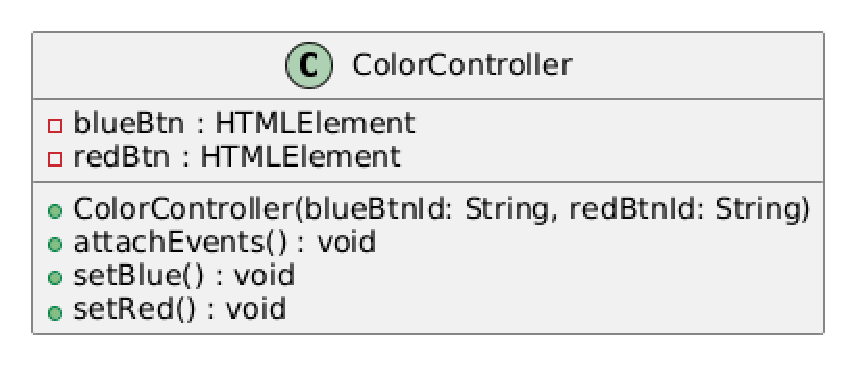
\includegraphics[width=0.6\linewidth]{eps/ColorControllerUML.eps}
  \caption{UML Class Diagram for the \texttt{ColorController} class}
  \label{fig:uml-colorcontroller}
\end{figure}
